\chapter{系统案例测试分析}

本节旨在展示系统在自然语言驱动的交通场景生成任务中的实际运行效果,我将拓展对案例的分析测试,从纵向和横向两个方面分析生成的效果。通过选取多个具有代表性的输入示例,分别涵盖了不同类型的交通语义指令,如静态车道场景、红绿灯交叉口、雨天行车、复杂车辆交汇等,全面体现系统在语义理解、场景构建、三维仿真以及评估反馈等方面的功能表现。

每一个示例均从用户界面输入开始,系统首先对自然语言进行语义编码与理解,然后通过检索模块筛选相关的语义片段或模板,接着由生成模块构造结构化的 Scenic 脚本,最终由 Carla 仿真环境还原为三维可视化场景。系统自动捕捉仿真结果图像,并结合评估模块生成语义一致性、多样性、结构完整性等量化指标,综合展示该场景的构建质量。
\section{场景案例测试}
为了验证系统生成场景是否具备多样性与高保真性,本章节会展示若干个典型的测试场景,这些场景涵盖红绿灯等待、夜间行驶等真实交通情境,每个场景都是由自然语言输入来生成的,并且会在CARLA仿真平台当中运行从而得到图像结果,通过这些实例能够直观观察系统对不同语义描述的解析能力,还有最终生成场景所呈现出的真实感与复杂度。



\subsection{场景一:自车在道路上行驶时,一名行人突然从左侧前方穿出}
用户自然语言输入:The ego vehicle is driving on a road when a pedestrian suddenly crosses from the left front and suddenly stops as the ego vehicle approaches.

\vspace{1em}

\begin{figure}[H]
	\centering
	\begin{minipage}[t]{0.48\textwidth}
		\centering
		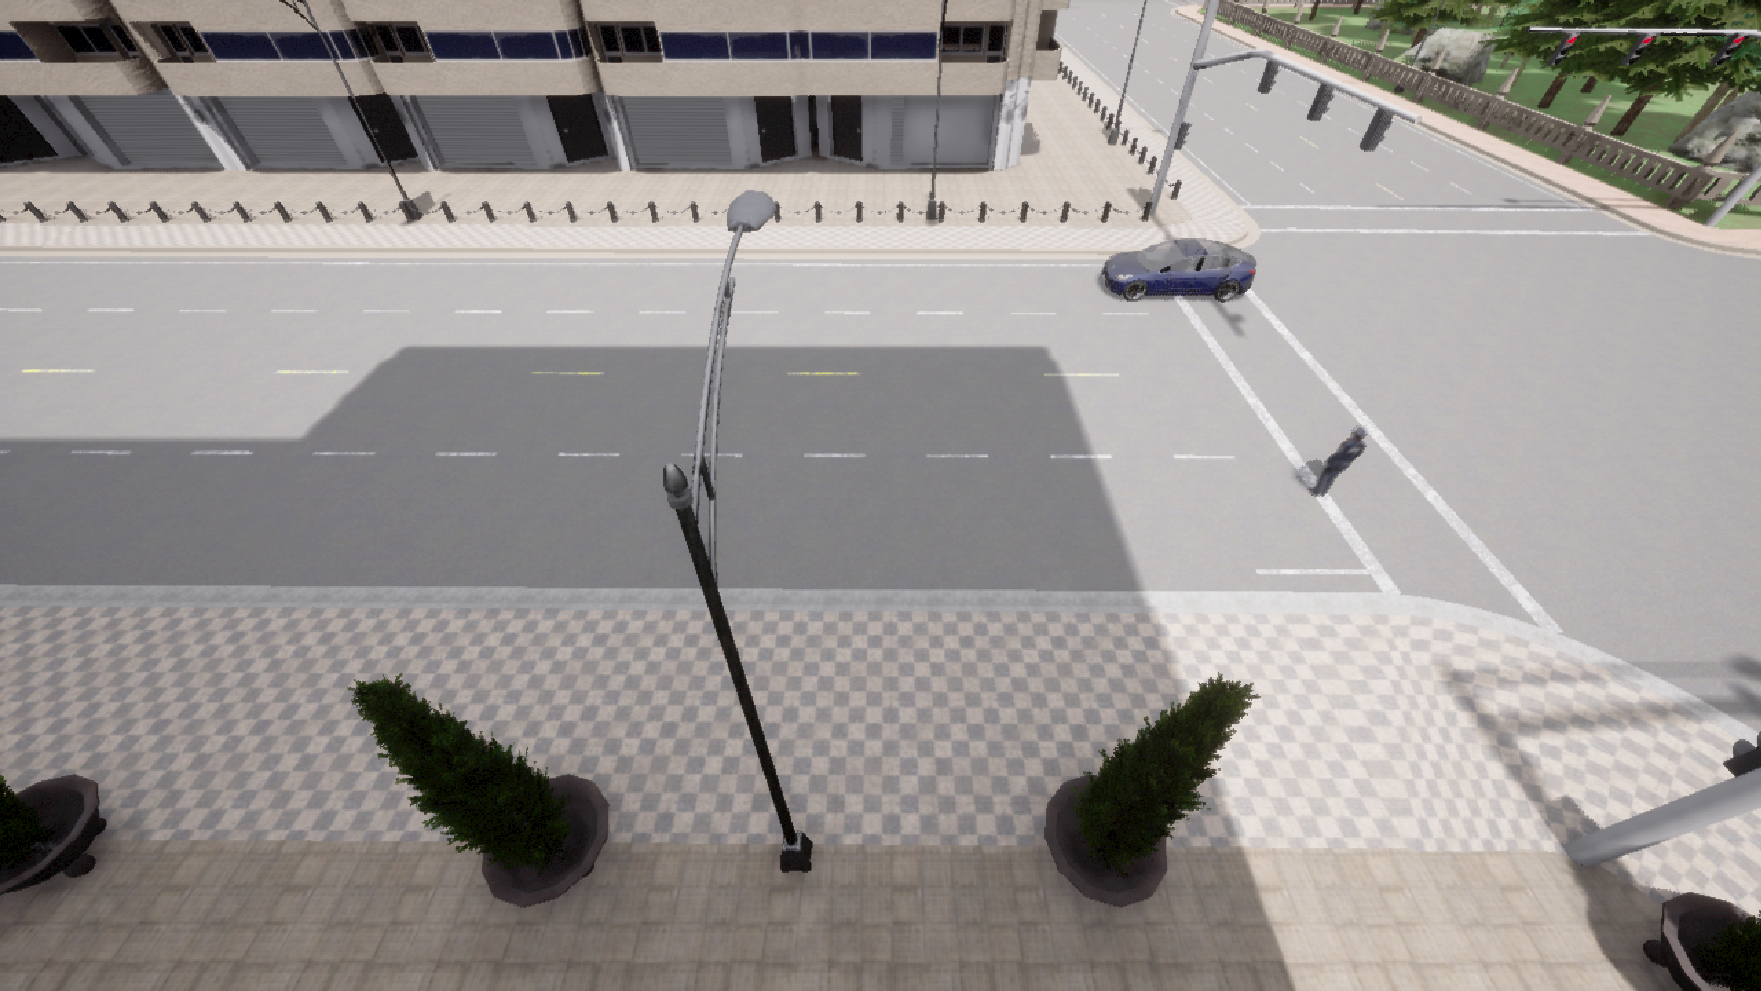
\includegraphics[width=\linewidth]{"images/场景6.pdf"}
		\caption{行人从左侧前方穿出 - 视角一}
		\label{fig:scene6_1}
	\end{minipage}%
	\hfill
	\begin{minipage}[t]{0.48\textwidth}
		\centering
		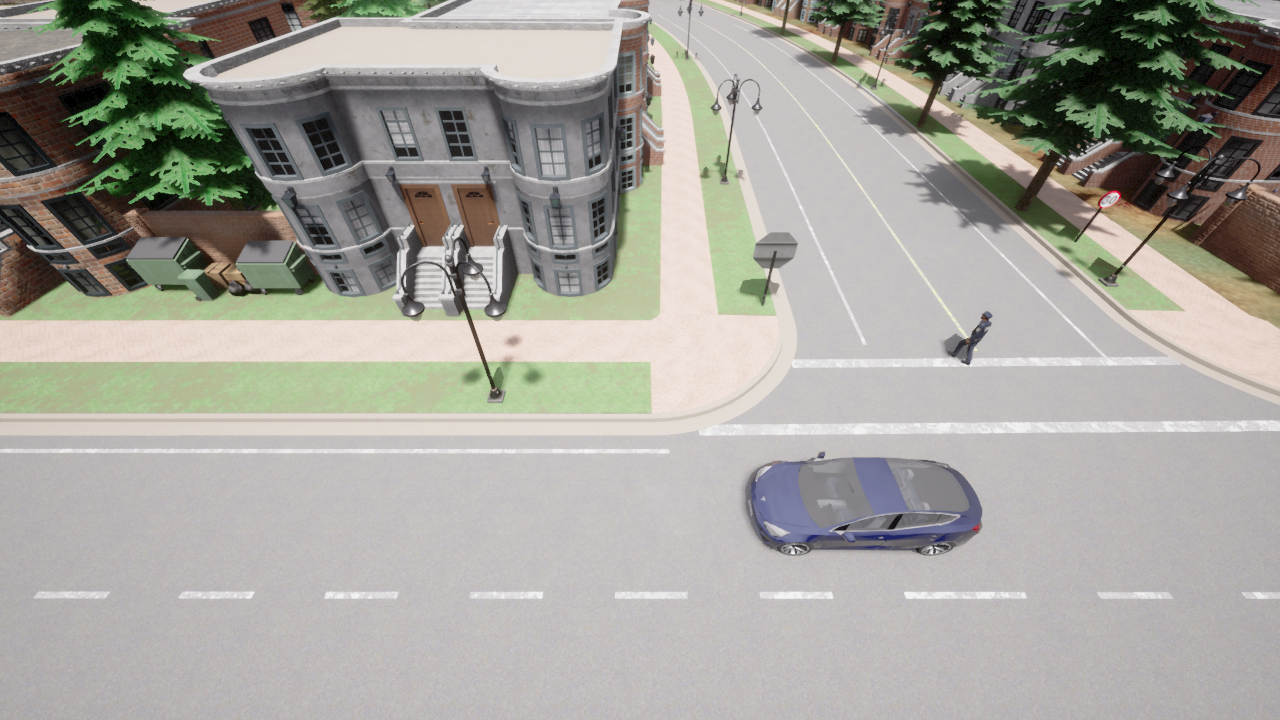
\includegraphics[width=\linewidth]{"images/场景6.1.png"}
		\caption{行人从左侧前方穿出 - 视角二}
		\label{fig:scene6_2}
	\end{minipage}
\end{figure}
从横向对比来看,每一次场景生成,都会有一定的变动与误差,在这个场景中,自车与行人的相对位置在生成的时候会有差异。分析原因可能有,当车速与行人的相对速度过大时会造成生成出来的效果偏差。
\subsection{场景二:两辆自车在直路上前后行驶}
用户自然语言输入:Two ego vehicles are driving in a straight line, one following the other.

\vspace{1em}

\begin{figure}[H]
	\centering
	\begin{minipage}[t]{0.48\textwidth}
		\centering
		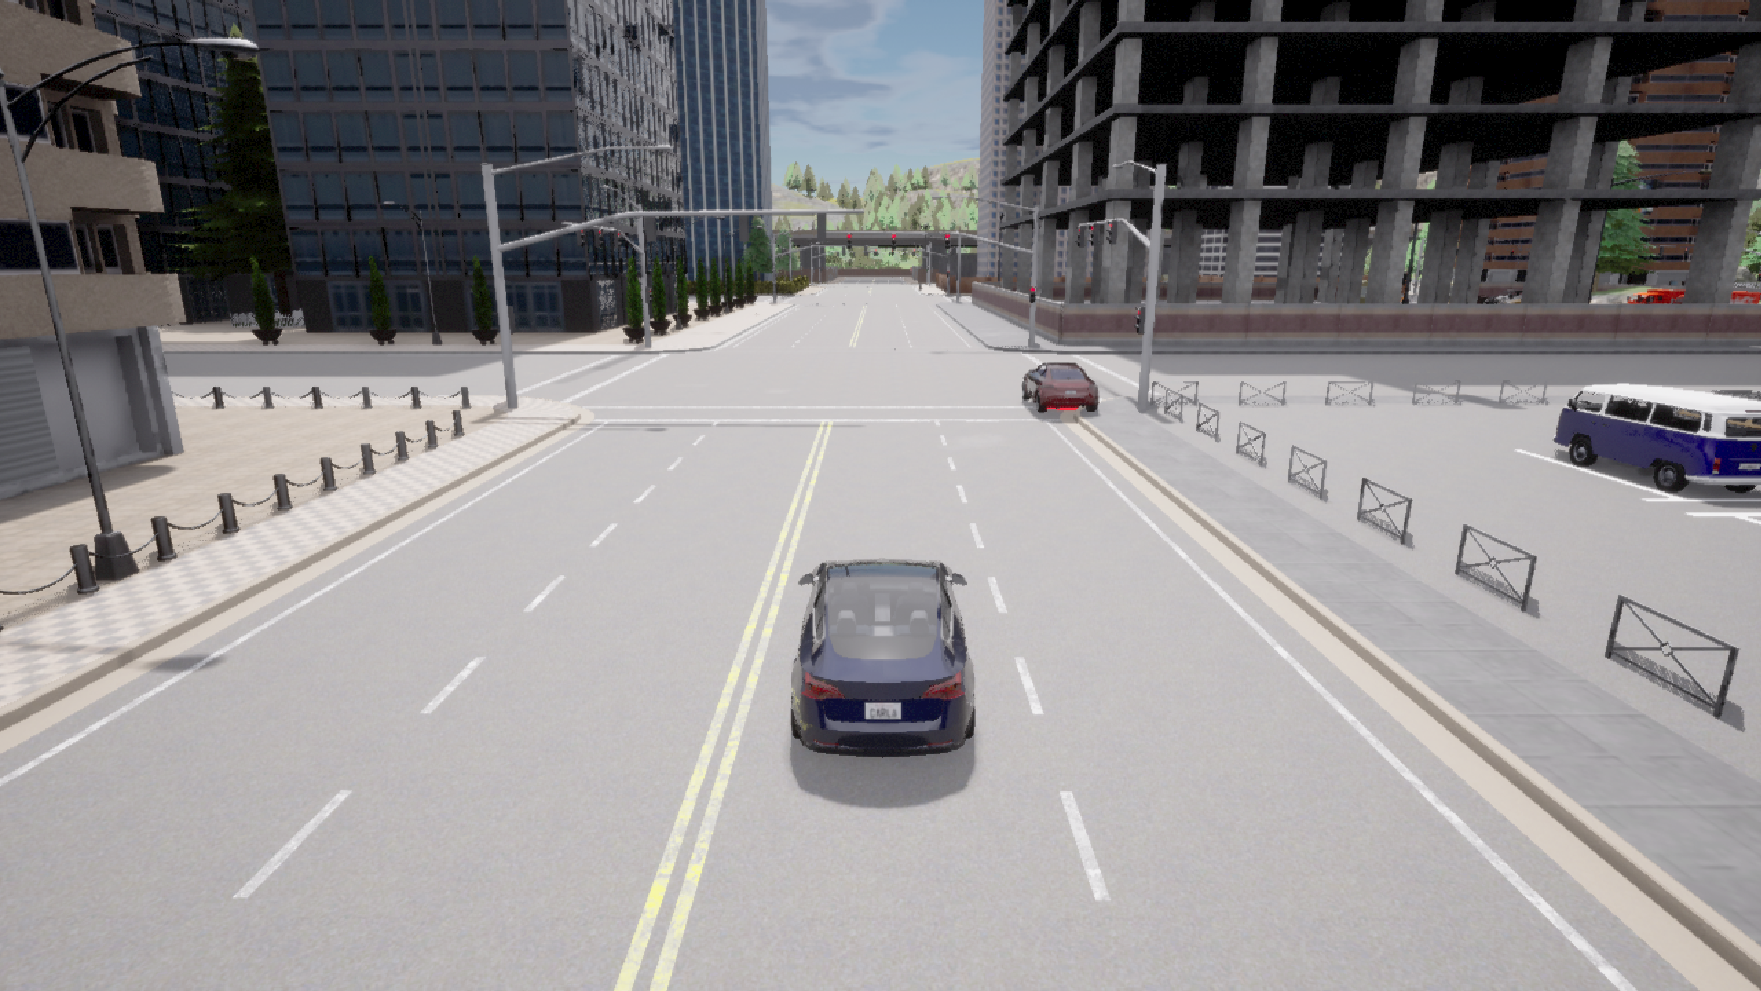
\includegraphics[width=\linewidth]{"images/场景7.pdf"}
		\caption{两辆自车直线行驶 - 视角一}
		\label{fig:scene7_1}
	\end{minipage}%
	\hfill
	\begin{minipage}[t]{0.48\textwidth}
		\centering
		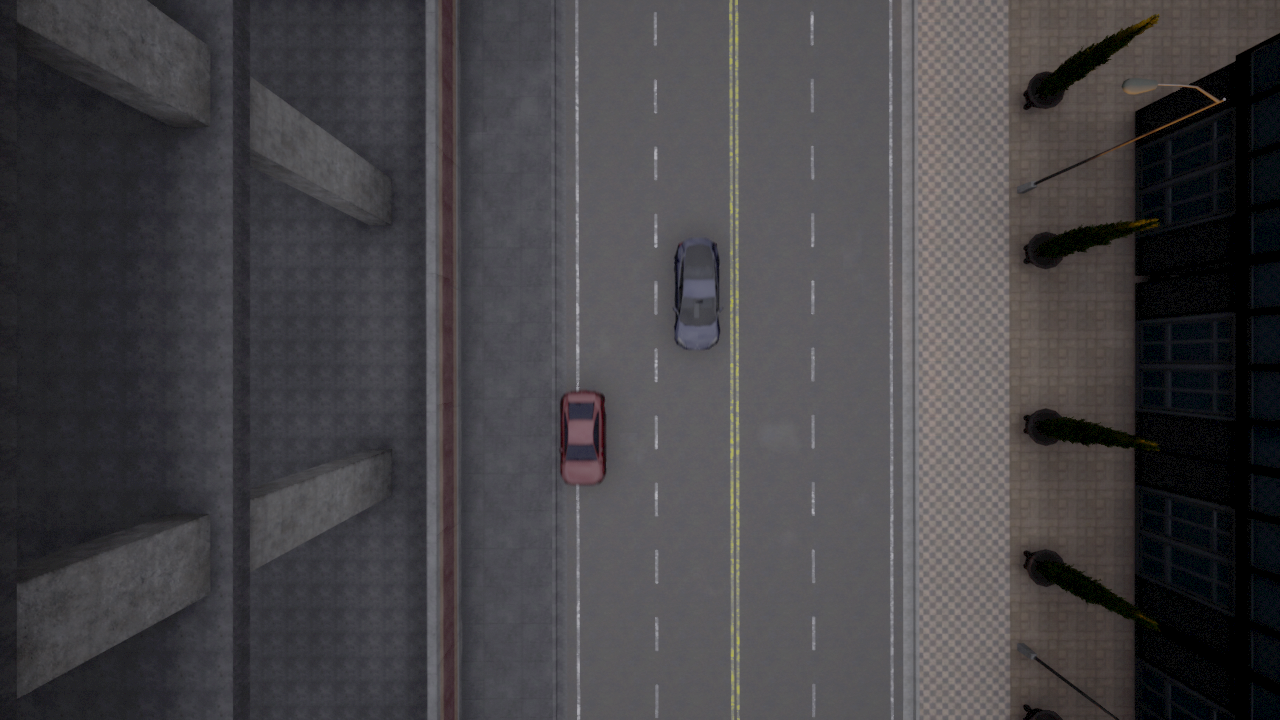
\includegraphics[width=\linewidth]{"images/场景7.1.png"}
		\caption{两辆自车直线行驶 - 视角二}
		\label{fig:scene7_2}
	\end{minipage}
\end{figure}
在本次对比中可以看出,视角的选取不同,也会影响效果的差异,所以调用相机的模块在场景生成中也十分重要。
\subsection{场景三:一名行人横穿马路而自车在直路上行驶}
用户自然语言输入:A ego vehicle is driving on a straight road while a pedestrian is crossing the street.

\vspace{1em}

\begin{figure}[H]
	\centering
	\begin{minipage}[t]{0.48\textwidth}
		\centering
		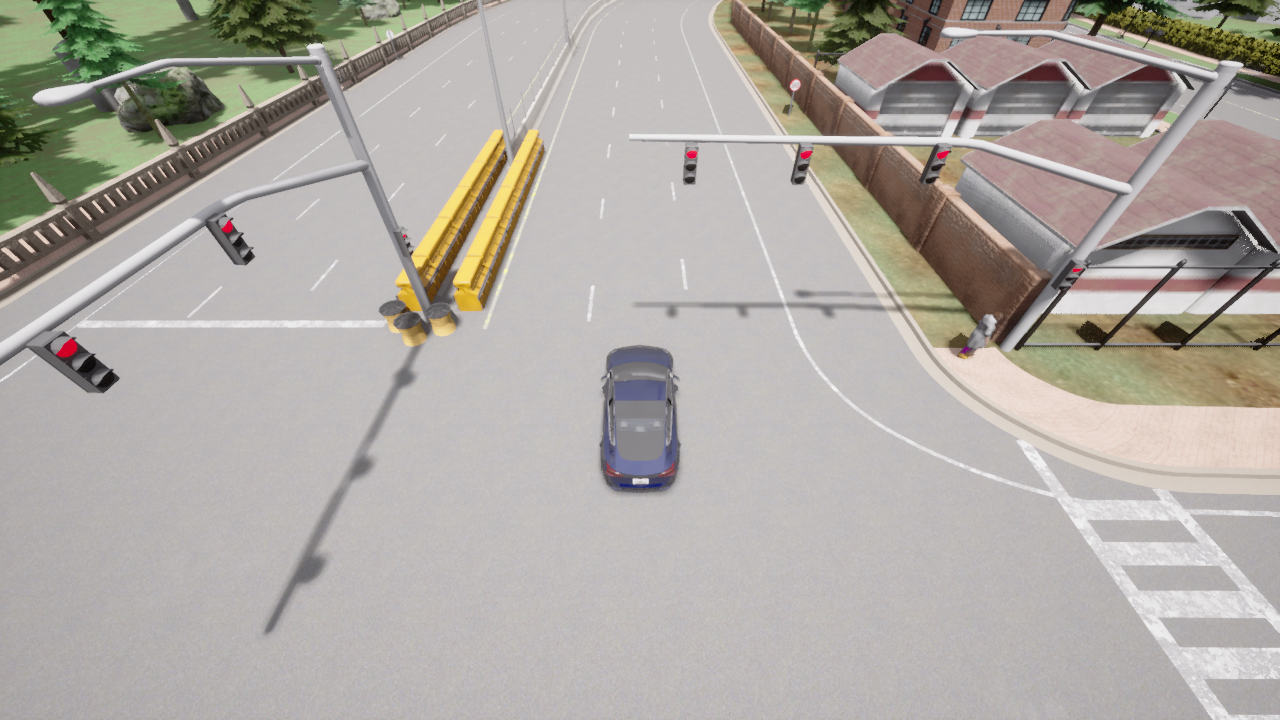
\includegraphics[width=\linewidth]{"images/场景10.pdf"}
		\caption{行人横穿马路 - 视角一}
		\label{fig:scene8_1}
	\end{minipage}%
	\hfill
	\begin{minipage}[t]{0.48\textwidth}
		\centering
		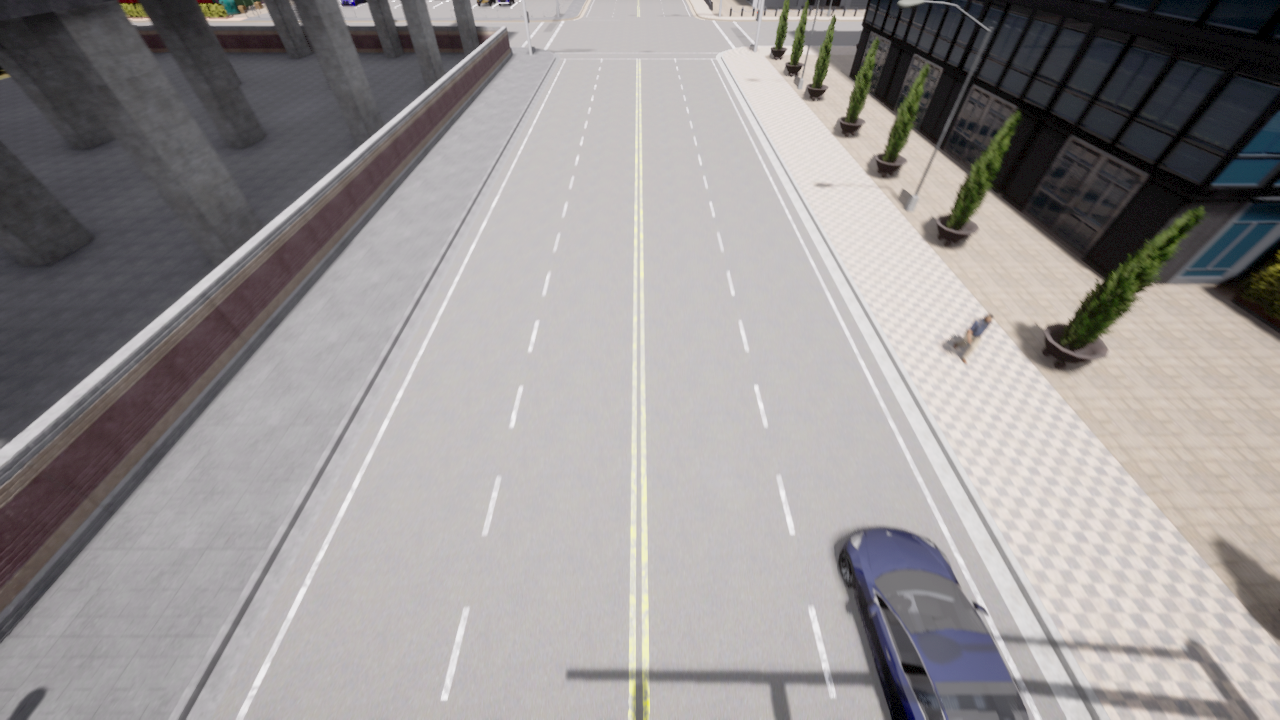
\includegraphics[width=\linewidth]{"images/场景8.1.png"}
		\caption{行人横穿马路 - 视角二}
		\label{fig:scene8_2}
	\end{minipage}
\end{figure}

\subsection{场景四:夜晚行人在人行道上走}
用户自然语言输入:\indent At night, a pedestrian is walking on the sidewalk.\\

\begin{figure}[H]
	\centering
	\begin{subfigure}[t]{0.48\textwidth}
		\centering
		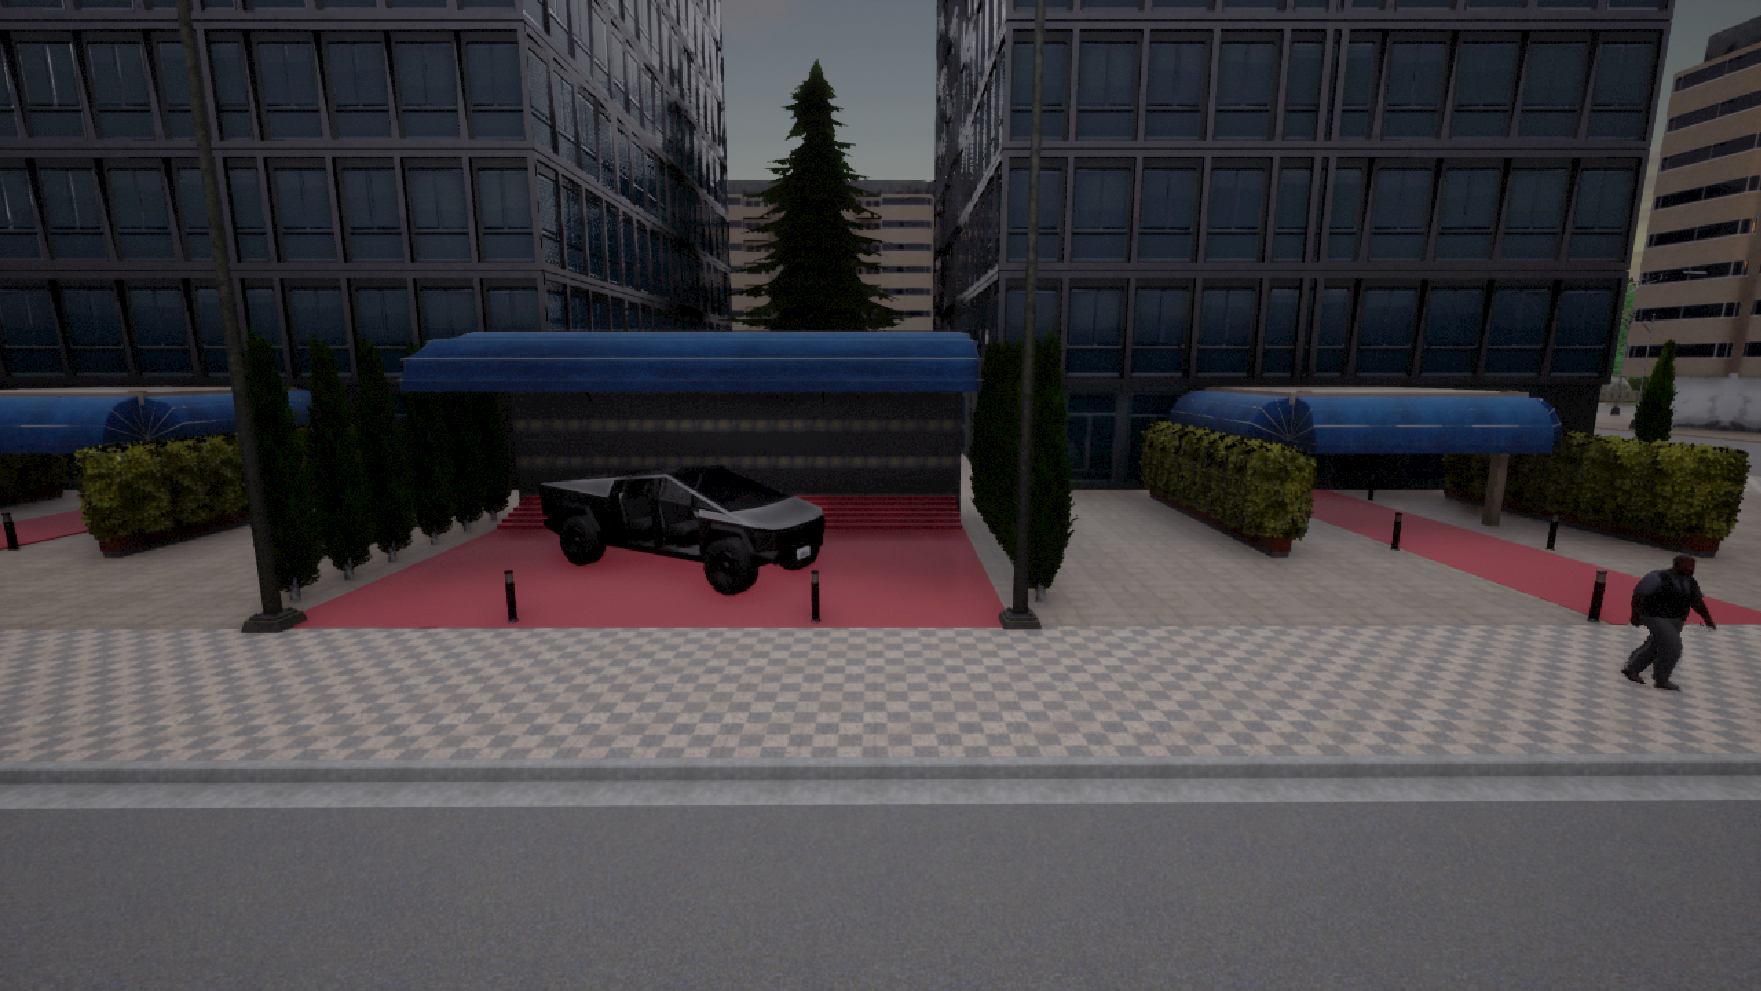
\includegraphics[width=\textwidth]{images/场景9.pdf}
		\caption{}
		\label{fig:night_sidewalk_1}
	\end{subfigure}
	\hfill % 添加一些水平间距
	\begin{subfigure}[t]{0.48\textwidth}
		\centering
		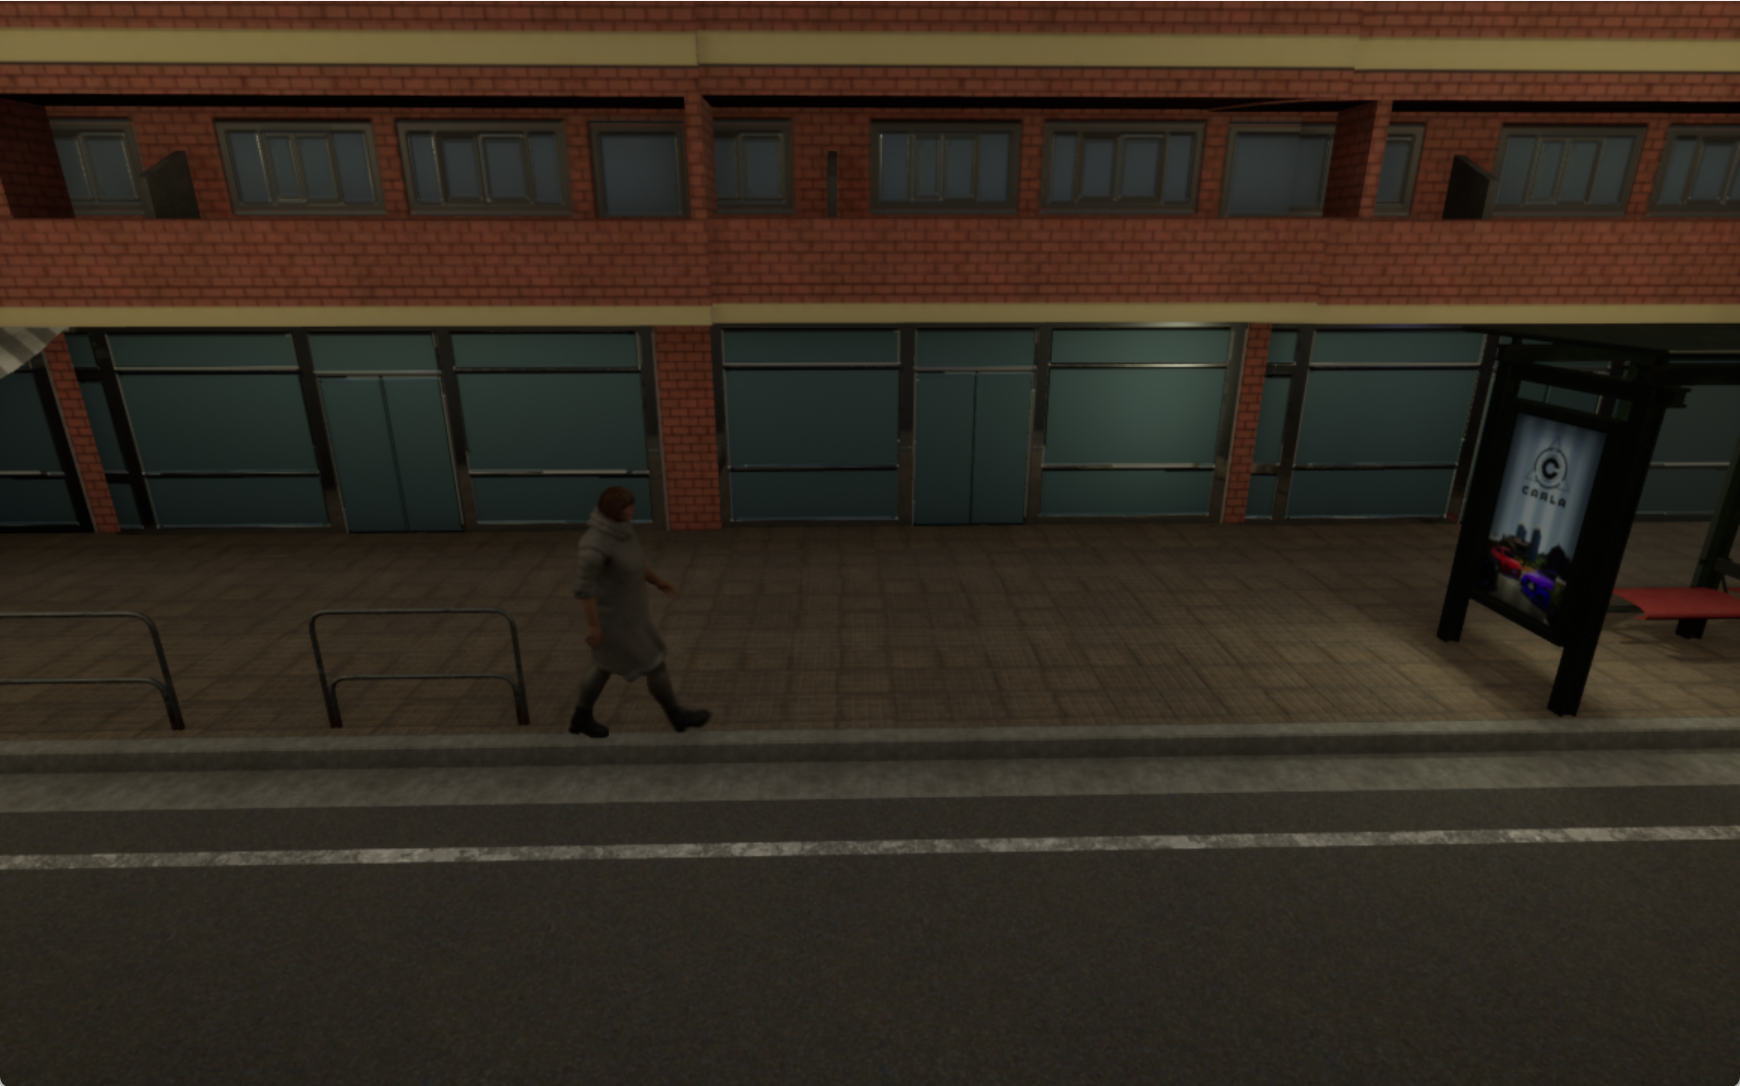
\includegraphics[width=\textwidth]{images/场景9.1.png}
		\caption{}
		\label{fig:night_sidewalk_2}
	\end{subfigure}
	\caption{夜晚行人在人行道上走}
	\label{fig:night_sidewalk}
\end{figure}
该场景展示了横向对比中生成的行人运动状态也会有所不同,证明对目标主体的状态描述可以更加详尽。
\subsection{场景五:自车通过十字路口}
用户自然语言输入:\index The ego vehicle passes through the intersection.\\

\begin{figure}[H]
	\centering
	\begin{subfigure}[t]{0.48\textwidth}
		\centering
		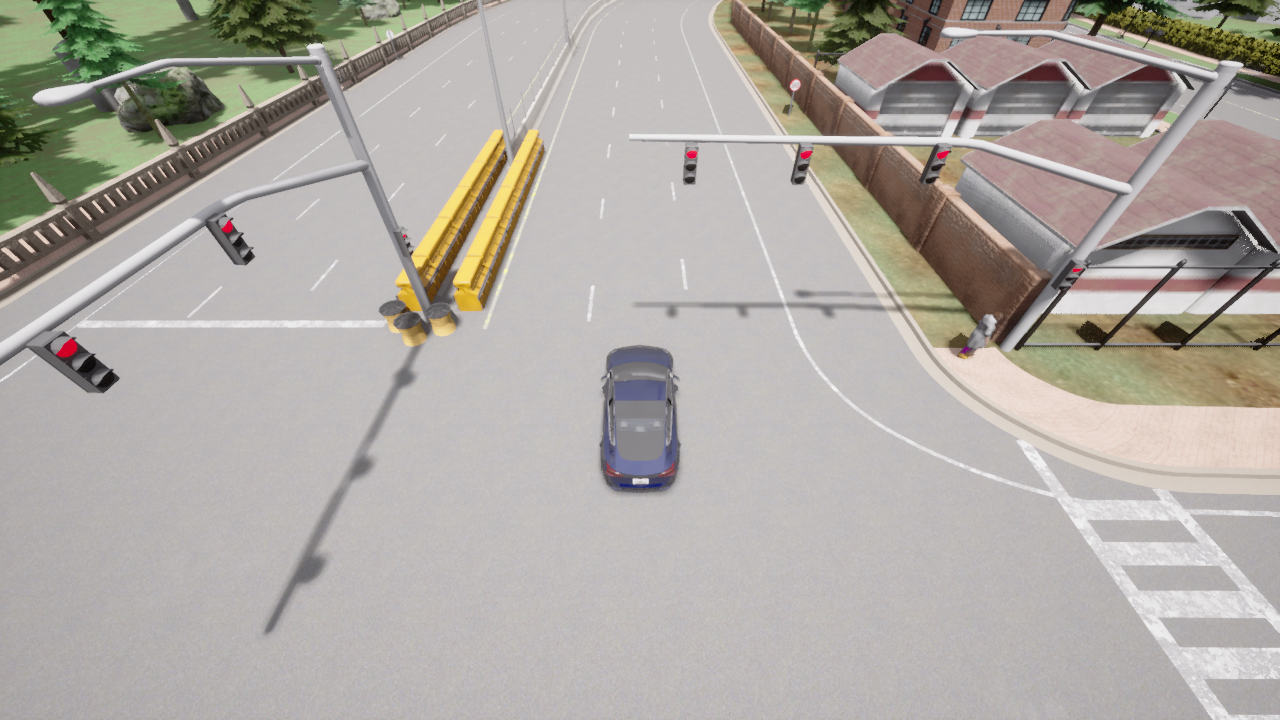
\includegraphics[width=\textwidth, height=0.8\textwidth, keepaspectratio]{images/场景10.png}
		\caption{}
		\label{fig:scene10-1}
	\end{subfigure}
	\hfill % 添加水平间距
	\begin{subfigure}[t]{0.48\textwidth}
		\centering
		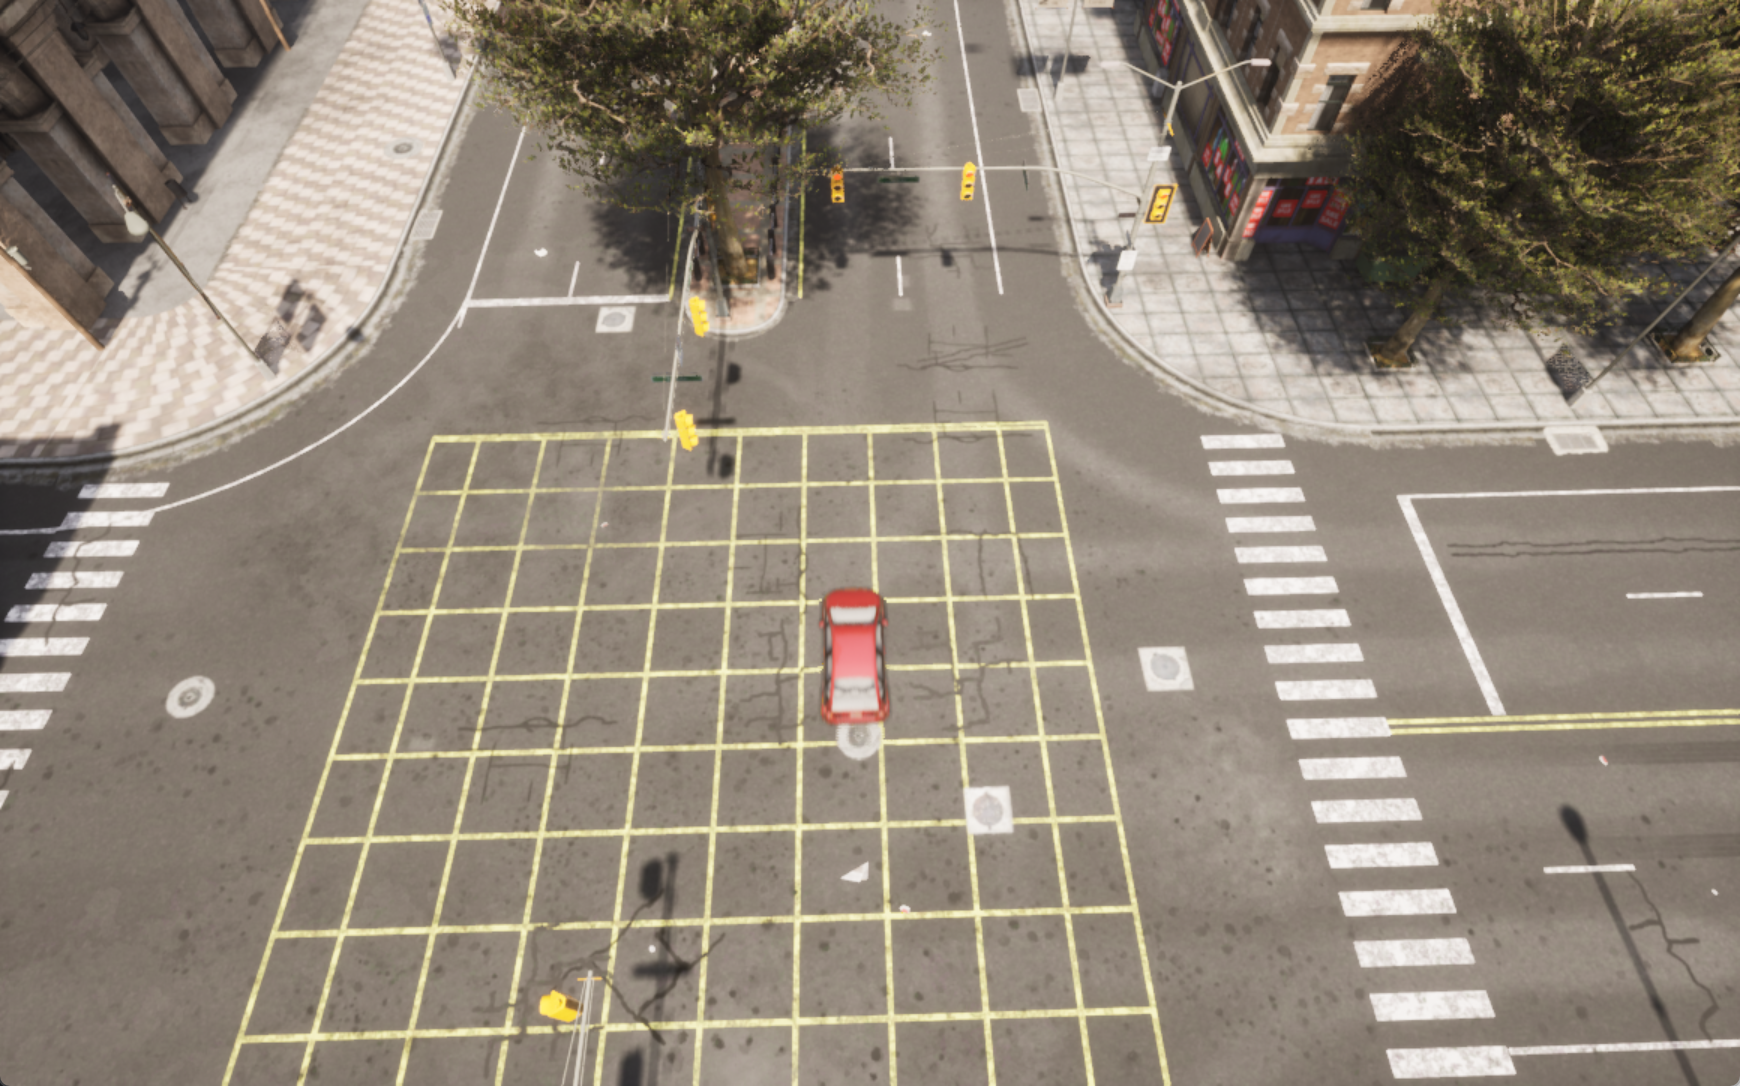
\includegraphics[width=\textwidth, height=0.8\textwidth, keepaspectratio]{images/场景10.1.png}
		\caption{}
		\label{fig:scene10-2}
	\end{subfigure}
	\caption{自车通过十字路口}
	\label{fig:scene10}
\end{figure}
场景五展示了town1和town5中运行代码的效果。

\section{评估测试分析}
为全面、客观地衡量本系统在从自然语言生成高保真三维交通场景过程中的表现,本文从语义保真度、场景多样性与系统效率三个核心维度构建了一套评估体系,具体指标设计如下:

(1)语义保真度(Semantic Fidelity):它主要是评估生成场景能不能准确还原输入自然语言里的核心语义信息,以此确保系统生成结果在语义层面有一致性和完整性。评估内容包含参与主体的一致性,像描述里提到的车辆类型比如红色轿车、卡车,还有行人、障碍物是否出现在仿真场景当中,空间位置关系,例如“在路口等待”“位于右侧车道”“靠近斑马线”等描述是否体现在实体布局里面,行为逻辑一致性,比如“等待绿灯”“直行通过”“与前车保持车距”等行为是否在仿真中能体现出来。评估方式采用检索式语义匹配评分也就是自动化加上人工评审打分也就是主观验证的双重手段,自动化方面是用自然语言处理模型计算输入描述和生成场景之间的语义相似度,主观方面是由3名评估者依据统一评分标准对每条样本进行1到5分打分,然后取平均作为最终得分。

(2)场景多样性(Scene Diversity):多样性评估用于衡量系统在面对不同自然语言输入时所生成场景之间的差异性,防止生成内容趋于模板化或重复模式。主要从以下几个角度度量:
1.结构多样性(Structure Diversity Score, SDS):通过提取场景中的车辆、行人、建筑等静态元素的布局特征,计算不同场景之间的结构差异程度;

2.行为多样性(Behavioral Diversity Score, BDS):通过仿真轨迹分析车辆在不同行为状态(加速、刹车、等待、避让等)上的变化情况,评估其动态多样性;

3.地图覆盖率方面要统计不同输入生成场景在CARLA地图里的分布情况,以此评估是否存在特定区域集中度过高的问题,采用像结构差异率、行为状态熵等定量指标来开展自动化评估工作,并且结合统计图表做可视化展示。

(3)系统效率与响应能力(Efficiency):系统效率是衡量该平台在真实应用场景下可行性的重要指标,重点考察系统从接收自然语言指令到输出完整三维场景所需的总时间开销,包括:检索耗时:Sentence-T5 向量化及相似描述查找所用时间;生成耗时:大语言模型生成 Scenic 脚本所耗时间;仿真加载与渲染时间:Scenic 编译后至 CARLA 仿真运行启动所经历的延迟;总响应时间:综合上述所有子流程,从输入自然语言到仿真画面出现的端到端时间。

通过日志记录还有脚本打点的方式来采集各个阶段的耗时,并且用平均响应时长(ms)、方差这类指标对性能表现进行量化,系统在多轮连续输入情况下的响应稳定性也被纳入评估范围。

在评估生成场景的质量时本研究选两种有代表性方法作基线对比,基于规则的方法即Rule - based这种方法通过定义明确逻辑和规则生成场景,它具有较好可解释性适合处理结构化和预定义任务,不过面对复杂和模糊的自然语言描述时灵活性和适应性较差,基于GPT - 4.0的方法借助大型语言模型生成能力来生成丰富多样的场景,该方法在场景生成多样性方面具备优势,不过在生成场景的物理合规性和逻辑一致性上存在不足,尤其是在处理复杂交通情境的时候。
选择这两种基线的主要目的是从不同角度评估本研究方法在生成场景质量、效率以及针对复杂和模糊指令的鲁棒性方面所具备的优势。\\




平均得分为 4.38,说明生成系统在语义还原方面表现优异,能够较好地捕捉自然语言中的关键词及其空间/行为语义。

\subsection{准确率分析}
在输入条件近似的情况下,系统生成了具有多样参与者布局与动作的场景。采用结构特征编码后计算场景间欧几里得距离,多样性指标如 碰撞率、闯红灯频率、停车标志频率、超出道路长度、路线跟随稳定性、路线完成率、平均花费时间、平均加速度、平均偏航速度以及车道入侵频率等,下面两张图通过横向对比,同一场景生成的结果分析会有所不同,但最后得出final Score保持在0.94-0.95之间,说明系统具备良好的准确率\ref{tab:evaluation_results}。
此外,通过对生成的截图进行视觉对比,发现系统在车辆类型、行驶方向、光照与天气等维度的变化也具备一定随机性与可控性。以下为两个评估测试的结果截图:
\begin{table}[H]
	\centering
	\begin{tabular}{|l|c|}
		\hline
		\textbf{Evaluation Metric} & \textbf{Value} \\
		\hline
		Collision Rate (碰撞率) & 0.0 \\
		\hline
		Avg. Red Light Frequency (平均闯红灯频率) & 0.0 \\
		\hline
		Avg. Stop Sign Frequency (平均停车标志频率) & 0.0 \\
		\hline
		Out-of-Road Length (超出道路长度) & 0.0 \\
		\hline
		Route Following Stability (路线跟随稳定性) & 0.8954 \\
		\hline
		Route Completion (路线完成率) & 0.9932 \\
		\hline
		Avg. Time Spent (平均花费时间) & 6.0342 \\
		\hline
		Avg. Acceleration (平均加速度) & 0.687 \\
		\hline
		Avg. Yaw Velocity (平均偏航速度) & 0.0 \\
		\hline
		Avg. Lane Invasion Frequency (平均车道入侵频率) & 0.0 \\
		\hline
		Safety OS (安全操作系统) & 1.0 \\
		\hline
		Task OS (任务操作系统) & 0.6863 \\
		\hline
		Comfort OS (舒适操作系统) & 1.0000 \\
		\hline
		Final Score (最终得分) & 0.9519 \\
		\hline
	\end{tabular}
	\caption{Evaluation Results1}
	\label{tab:evaluation_results}
\end{table}

\begin{table}[H]
	\centering
	\begin{tabular}{|l|c|}
		\hline
		\textbf{Evaluation Metric} & \textbf{Value} \\
		\hline
		Collision Rate (碰撞率) & 0.0 \\
		\hline
		Avg. Red Light Frequency (平均闯红灯频率) & 0.0 \\
		\hline
		Avg. Stop Sign Frequency (平均停车标志频率) & 0.0 \\
		\hline
		Out-of-Road Length (超出道路长度) & 0.0 \\
		\hline
		Route Following Stability (路线跟随稳定性) & 0.8542 \\
		\hline
		Route Completion (路线完成率) & 0.9865 \\
		\hline
		Avg. Time Spent (平均花费时间) & 5.325 \\
		\hline
		Avg. Acceleration (平均加速度) & 0.7869 \\
		\hline
		Avg. Yaw Velocity (平均偏航速度) & 0.0 \\
		\hline
		Avg. Lane Invasion Frequency (平均车道入侵频率) & 0.0 \\
		\hline
		Safety OS (安全操作系统) & 1.0 \\
		\hline
		Task OS (任务操作系统) & 0.6934 \\
		\hline
		Comfort OS (舒适操作系统) & 1.0000 \\
		\hline
		Final Score (最终得分) & 0.9409 \\
		\hline
	\end{tabular}
	\caption{Evaluation Results2}
	\label{tab:evaluation_results2}
\end{table}

\subsection{效率分析}
系统整体生成流程的平均时间如下:


为了评估基于自然语言生成高保真智能驾驶仿真场景系统的整体性能,我们把完整流程划分成五个主要的阶段,并且针对每一阶段的平均运行时间、关键输出结果以及其影响因素进行了详细统计与分析,具体内容如表 \ref{tab:simulation_time} 所示。
\begin{table}[H]
	\centering
	\renewcommand{\arraystretch}{1.2}
	\begin{tabular}{p{4cm} p{2.5cm} p{2.8cm} p{4.5cm}}
		\hline
		\textbf{阶段} & \textbf{平均时间 (秒)} & \textbf{关键输出} & \textbf{影响因素 / 可调参数} \\
		\hline
		语义检索与匹配 & 1.6 & 相似场景向量 + 匹配索引 & 检索库规模、向量维度、匹配阈值、Top-K 设置 \\
		Scenic 脚本生成 & 2.3 & Scenic 场景脚本 (.scenic) & 场景模板复杂度、语言理解精度、地形元素数量 \\
		Scenic 到配置转换 & 0.7 & .config 配置文件 & 转换规则数量、是否包含动态目标 \\
		Carla 场景加载与构建 & 3.2 & Carla 世界状态 & 地图大小、天气设置、对象密度 \\
		截图渲染与保存 & 1.1 & RGB 图像 (.png) & 分辨率、渲染设备性能、截图角度 \\
		\hline
		\textbf{总耗时} & \textbf{8.9} & --- & 与系统性能、并发线程数等有关 \\
		\hline
	\end{tabular}
	\caption{自然语言生成场景的各阶段性能统计}
	\label{tab:simulation_time}
\end{table}
首先语义检索与匹配阶段的主要任务是把用户输入的自然语言描述转化成向量表示,然后和预先构建好的场景语义向量库进行相似度检索,这个阶段平均耗费时间大约为1.6秒,输出的内容是一组相似场景的索引以及向量,其主要受到检索库规模、向量维度、匹配阈值还有Top - K值设置等因素的影响 。

其次在Scenic脚本生成阶段会把检索到的匹配结果和语言模板相结合,进而自动构造出符合语义的.scenic脚本,此阶段平均耗时为2.3秒,该阶段的耗时会受到场景描述复杂程度、地形构造模板数量、语言解析精度等因素的影响,特别是在涉及多个车辆与动态目标的情况下,脚本生成时间会有所上升。

接下来进入Scenic到配置转换这个阶段,此阶段会把.scenic文件解析成Carla兼容的.config配置文件,以此为后续仿真环境加载做好准备,这一过程平均需要花费0.7秒时间,处理逻辑相对来说比较轻量,转换规则的具体数量以及是否包含动态对象像自动驾驶目标车辆、行人等会略微对耗时产生影响。

第四阶段在整个流程里是最耗时间的部分,具体为Carla场景加载与构建,此阶段涵盖场景地图加载、静态和动态对象放置、交通信号配置等操作,平均所花费的时间是3.2秒,该阶段的性能很大程度上依赖于地图的大小、环境的复杂程度(像是否包含天气、光照等因素)以及硬件图形性能。

最后,截图渲染与保存阶段会调用Carla客户端API截取仿真视角下RGB图像并保存,此阶段平均耗时为1.1秒,影响因素包含图像分辨率、摄像机角度以及渲染硬件性能等。
从整体情况来看整个从自然语言输入到仿真图像输出流程平均耗时大概8.9秒,在单线程运行模式下已经具备比较不错的响应性能,要是进一步采用并发优化或者异步渲染技术,该系统在未来能够扩展成支持实时交互与多轮问答生成的智能仿真平台。
经实验验证,在一次性处理20条自然语言输入的情形下,系统可在不显著增加响应时间的前提下完成全部场景的构建与仿真,平均每个场景的处理时间波动控制在±0.7秒范围内。
这表明:

(1)系统核心模块间的异步处理与缓存机制有效;

(2)大语言模型调用延迟已通过缓存和批处理策略优化;

(3) Scenic 与 CARLA 接口连接在高频调用场景下仍保持稳定。

总体来说系统拥有良好响应效率和可扩展性,不但支持单条交互式输入方式,而且能够满足批量生成相关需求,适合大规模自动驾驶测试等实际应用任务,比如仿真训练或者仿真场景库构建等,若要进一步提升系统的运行效率,可通过这些途径来进行优化:引入本地轻量化大模型以减少云端调用延迟;对检索模块进行并行化改造,提升向量查找速度;使用CARLA的异步仿真接口或地图预加载技术降低启动时间。


\section{本章小节}
这章借助多个典型自然语言驱动交通场景案例,系统全面地展示本系统在语义理解、场景生成、三维仿真以及评估反馈等方面整体能力,实验结果显示系统可准确捕捉输入指令里核心语义信息,生成高保真度的三维交通场景,并且在车辆行为、环境光照、行人动作等细节上呈现出良好多样性与合理性,通过语义保真度和多样性两大核心指标量化评测,系统在语义一致性和场景丰富性方面都取得优异成绩。
此外系统在响应效率方面展现出较强实时性和稳定性,平均单条场景生成时间能控制在9秒以内,还支持批量输入处理,适合大规模自动驾驶仿真应用,基于规则方法和基于大语言模型方法对比验证,进一步凸显本系统在灵活性和复杂场景处理上的优势。综上所述本章测试分析充分证明本系统在自然语言到三维智能驾驶场景自动生成领域有效性与实用价值,为后续系统优化和应用推广奠定坚实基础。












